\section{Communication from the shell- to the remote-application}\label{section:methods:communication-shell-remote}

To solve the problem of building a common caching layer, some form of communication between the shell and remote application had to be implemented. To ensure that the micro-frontends remain independent of each other, it should be avoided that they communicate directly with each other.

Angular provides a great tool for this use case, namely dependency injection. The shell application can provide services that can later be injected by the remote applications. This is very handy because the micro frontend can provide the same services as the shell application in standalone mode. Therefore, the remote module can be easily used within the remote and shell application.

For example i implemented a layout-service that takes advantage of dependency injection.

\ifshowImages
\begin{figure}[H]
\centering

\includegraphics[width=1\linewidth]{images/prototype-screenshots/contact-header.png}
\caption{Beispiel für die Beschriftung eines Buchrückens.}
\end{figure}
\fi

\ifshowImages
\begin{figure}[H]
\centering
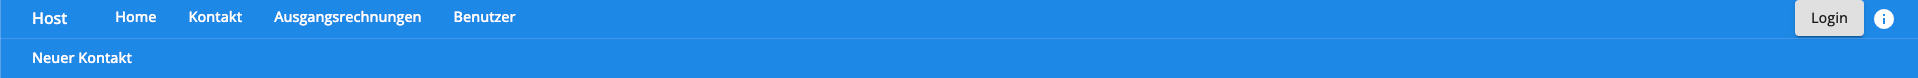
\includegraphics[width=1\linewidth]{images/prototype-screenshots/host-contact-header.png}
\caption{Beispiel für die Beschriftung eines Buchrückens.}
\end{figure}
\fi
